\section{Moduli of curve}
The content of this section is already well written in the course \href{https://johannesschmitt.gitlab.io/moduli_of_curves}{``the moduli space of curves"}. This section is just for the completeness of the survey. 

Maybe \cite{harris2006moduli} would be another good reference for this section, especially for the readers concerning about arithmetic. I haven't read about it.

So now comes the conclusion.
\subsection{Initial definition}
\begin{defn}[{smooth/stable curve, follow \cite[Definition 3.15]{modulicurve}}]
For $g,n \geqslant 0$, a smooth curve of genus $g$ over $S \in \Schk$ with $n$-points is an element in the set
$$\mathcal{A}_S:=\left\{(X,\pi,\sigma_i)  \;\middle|\; \begin{aligned}
&\\[-5mm]
&X \in \Ob(\Schk)\\[-1mm]
&\pi:X \longrightarrow S \text{ proper flat and }\\[-1mm]
&\hspace{1cm}\pi^{-1}(\Spec L) \text{ is a sm proj connected curve of genus $g$}\\[-1mm]
&\sigma_i:S \longrightarrow X \text{ pairwise disjoint sections of }\pi
\end{aligned}
 \right\}$$
 and a stable curve of genus $g$ over $S \in \Schk$ with $n$-points is an element in the set
 $$\overline{\mathcal{A}}_S:=\left\{(X,\pi,\sigma_i)  \;\middle|\; \begin{aligned}
 &\\[-5mm]
 &X \in \Ob(\Schk)\\[-1mm]
 &\pi:X \longrightarrow S \text{ proper flat \textcolor{gray}{(maybe not smooth)} }\\[-1mm]
 &\hspace{1cm}\pi^{-1}(\Spec L) \text{ is a \textcolor{red}{stable} proj connected curve of genus $g$}\\[-1mm]
 &\sigma_i:S \longrightarrow X \text{ pairwise disjoint sections of }\pi\\[-1mm]
 &\hspace{2.1cm}\text{ with image in the smooth locus of $\pi$}
 \end{aligned}
  \right\}$$
\end{defn}
\begin{defn}[moduli of smooth/stable curves]\label{def:moduliofcurves}
For $g,n \geqslant 0$, the moduli of smooth curves $\mathcal{M}_{g,n}$ and the moduli of smooth curves $\overline{\mathcal{M}}_{g,n}$ are defined as
$$\mathcal{M}_{g,n}(S)=\mathcal{A}_S/\sim_S \qquad \mathcal{M}_{g,n}(f:T\longrightarrow S)=f^*: \mathcal{A}_S/\sim_S \longrightarrow \mathcal{A}_T/\sim_T.$$
$$\overline{\mathcal{M}}_{g,n}(S)=\overline{\mathcal{A}}_S/\sim_S \qquad \overline{\mathcal{M}}_{g,n}(f:T\longrightarrow S)=f^*: \overline{\mathcal{A}}_S/\sim_S \longrightarrow \overline{\mathcal{A}}_T/\sim_T.$$
where the equivalent relation $\sim_S$ and the pullback are similar in the Example \ref{eg:M03}, i.e.
 $(X,\pi,\sigma_i) \sim_S (X',\pi',\sigma_i')$ if there exists an isomorphism $f:X \longrightarrow X'$ such that the following diagrams commute:
   % https://q.uiver.app/?q=WzAsNixbMCwwLCJYIl0sWzIsMCwiWCciXSxbMSwxLCJTIl0sWzMsMCwiWCJdLFs0LDEsIlMiXSxbNSwwLCJYJyJdLFszLDUsImYiXSxbNCw1LCJcXHNpZ21hX2knIiwyXSxbNCwzLCJcXHNpZ21hX2kiXSxbMCwyLCJcXHBpIiwyXSxbMSwyLCJcXHBpJyJdLFswLDEsImYiXV0=
   \[\begin{tikzcd}[column sep=3mm]
   	X && {X'} &[20mm] X && {X'} \\
   	& S &&& S
   	\arrow["f", from=1-4, to=1-6]
   	\arrow["{\sigma_i'}"', from=2-5, to=1-6]
   	\arrow["{\sigma_i}", from=2-5, to=1-4]
   	\arrow["\pi"', from=1-1, to=2-2]
   	\arrow["{\pi'}", from=1-3, to=2-2]
   	\arrow["f", from=1-1, to=1-3]
   \end{tikzcd}\]
   
   For a map $f:T \longrightarrow S$, the pullback $f^*$ is defined by
   $$f^*:\mathcal{A}_S \longrightarrow \mathcal{A}_T \qquad (X,\pi,\sigma_i) \longmapsto (X_T,\pi_T,\sigma_{i,T})$$
   where $X_T$, $\pi_T$ are defined as fiber product, and $\sigma_{i,T}$ are defined by the universal property of fiber product, as follows:
   % https://q.uiver.app/?q=WzAsOSxbMCwxLCJYX1QiXSxbMSwxLCJYIl0sWzAsMiwiVCJdLFsxLDIsIlMiXSxbMywxLCJYX1QiXSxbMywyLCJUIl0sWzQsMiwiUyJdLFs0LDEsIlgiXSxbMiwwLCJUIl0sWzAsMiwiXFxwaV9UIiwyXSxbMiwzLCJmIl0sWzEsMywiXFxwaSJdLFs0LDUsIlxccGlfVCIsMl0sWzUsNiwiZiJdLFs3LDYsIlxccGkiLDJdLFs0LDddLFs4LDcsIlxcc2lnbWFfaSBcXGNpcmMgZiIsMCx7ImN1cnZlIjotMn1dLFs4LDQsIlxcZXhpc3RzIFxcLCFcXCwgXFxzaWdtYV97aSxUfSAiLDAseyJsYWJlbF9wb3NpdGlvbiI6OTAsImNvbG91ciI6WzAsMTAwLDUwXSwic3R5bGUiOnsiYm9keSI6eyJuYW1lIjoiZGFzaGVkIn19fSxbMCwxMDAsNTAsMV1dLFs4LDUsIlxcSWRfVCIsMix7ImN1cnZlIjoyfV0sWzYsNywiXFxzaWdtYV97aX0iLDIseyJjdXJ2ZSI6MSwic3R5bGUiOnsiYm9keSI6eyJuYW1lIjoiZGFzaGVkIn19fV0sWzAsMV0sWzAsMywiIiwxLHsic3R5bGUiOnsibmFtZSI6ImNvcm5lciJ9fV0sWzQsNiwiIiwxLHsic3R5bGUiOnsibmFtZSI6ImNvcm5lciJ9fV1d
   \[\begin{tikzcd}
   	&&[15mm] T&[-6mm] \\[-6mm]
   	{X_T} & X && {X_T} & X \\
   	T & S && T & S
   	\arrow["{\pi_T}"', from=2-1, to=3-1]
   	\arrow["f", from=3-1, to=3-2]
   	\arrow["\pi", from=2-2, to=3-2]
   	\arrow["{\pi_T}"', from=2-4, to=3-4]
   	\arrow["f", from=3-4, to=3-5]
   	\arrow["\pi"', from=2-5, to=3-5]
   	\arrow[from=2-4, to=2-5]
   	\arrow["{\sigma_i \circ f}", curve={height=-12pt}, from=1-3, to=2-5]
   	\arrow["{\exists \,!\, \sigma_{i,T} }"{pos=1.12}, color=red, dashed, from=1-3, to=2-4]
   	\arrow["{\Id_T}"', curve={height=12pt}, from=1-3, to=3-4]
   	\arrow["{\sigma_{i}}"', curve={height=6pt}, dashed, from=3-5, to=2-5]
   	\arrow[from=2-1, to=2-2]
   	\arrow["\ulcorner"{anchor=center, pos=0.125}, draw=none, from=2-1, to=3-2]
   	\arrow["\ulcorner"{anchor=center, pos=0.125}, draw=none, from=2-4, to=3-5]
   \end{tikzcd}\]
\end{defn}
\subsection{Result}
Here is the result coming from \cite{modulicurve} which we really care: 
\begin{figure}[ht]
  \vspace{0cm}
    \centering  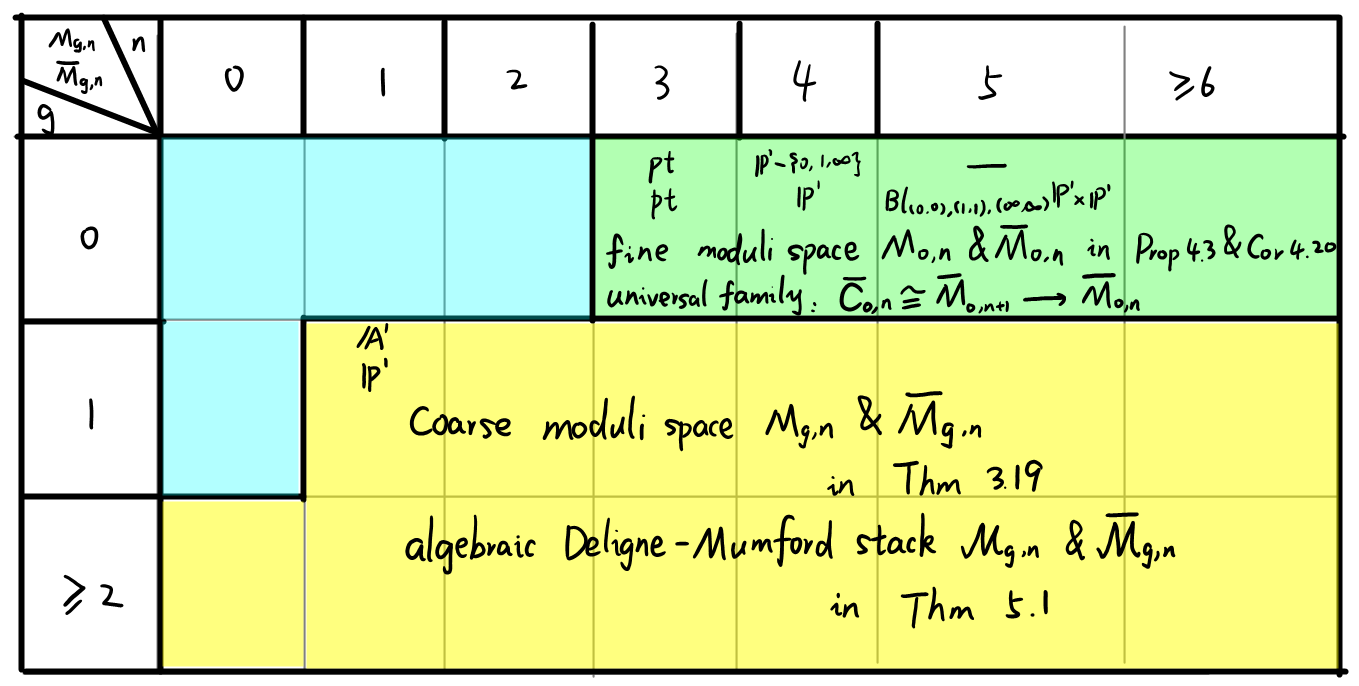
\includegraphics[width=12cm]{figures/moduliofcurve.png}
    \label{fig:moduliofcurve}
    \caption{The moduli of curves}
        
\end{figure} 

If you're interested on the automorphism of these moduli spaces, then you can check \cite{massarenti2013}. If you want to know the Euler characteristic of $\mathcal{M}_{g,n}$, you should check \cite{HZformula2021} for the Harer-Zagier formula.
%Which I haven't checked 